% !TEX encoding = UTF-8 Unicode
\documentclass[a4paper]{article}
\usepackage[utf8]{inputenc}
\usepackage[T1]{fontenc}
\usepackage[francais]{babel}
\usepackage{fullpage}
\usepackage{hyperref}
\usepackage{verbatim}
\usepackage{graphicx}
\usepackage[nonumberlist]{glossaries}
\usepackage{amssymb,amsmath}
\usepackage{subfig}
\usepackage{float}
\title{INFO-F404 - Real-Time Operating Systems\\Project 1: Global vs Partitioned DM}
\author{Anthony Caccia \and J\'{e}r\^{o}me Hellinckx}
\date{\today}

\begin{document}
\renewcommand{\labelitemi}{$\bullet$}
\maketitle

\section{Introduction}
This project consists in studying performances of the \emph{Deadline-monotonic scheduling} (DM) algorithm on systems with two different strategies : global and partitioned (best fit) scheduling. Systems have $n$ periodic, asynchronous and independant tasks $\tau$ with constrained deadlines on a multiprocessor system.

DM is a \emph{Fixed Task Priority Scheduler} (FTP) : tasks are ranked deterministically by their relative deadlines. The lower the relative deadline, the higher the priority. In case of equality, the priority still has to be deterministic. Therefore, in this implementation, the task id (which is unique) will decide of the priority.

\subsection{Partitioned strategy}
The main problem that has to be dealt with when using a partitioned strategy is to find an optimal partitioning such that each partition is schedulable on one processor while minimizing the number of partitions. Since this problem is known to be \emph{NP-Complete}, this implementation uses the best-fit heuristic algorithm to find a partitioning. The \emph{Best-Fit} strategy operates by assigning the current task to the processor for which the remaining utilization when adding said task utilization is minimum.

Once all tasks have been assigned to a partition, it cannot migrate and a uniprocessor scheduler is used on each partition. 

\subsection{Global strategy}
Global strategy, on the other hand, permits to tasks to migrate between processors during their lifetime : they can then start their execution on a processor and resume on another one.

\section{Code description}
Three executables were asked in order to complete this project:
\begin{enumerate}
  \item a simulator, taking as list of tasks, a number of processor and a strategy and simulate the system on the interval $I = [0; O_{max} + 2 * P]$;
  \item a generator, which creates a list of $n$ tasks with an utilization $u$;
  \item a study program, to test DM's performances.
\end{enumerate}

\subsection{Simulator}
Aside from the essential data types - \texttt{Task} and \texttt{Job} which are described in the files with corresponding names - needed by the scheduler, the simulator is fully defined by one main basic class (\texttt{PCDSimulator}) and two other classes (\texttt{PDMSimulator} and \texttt{GDMSimulator}) derived from said main class. The idea behind the abstract super class is to offer tools to facilitate the scheduling of systems of \underline{P}eriodic tasks with \underline{C}onstrained \underline{D}eadline (hence the name).
This base class achieves that in the following ways : 
\begin{itemize}
	\item Being a template class permitting to specify a priority comparator between jobs. This flexibility is quite powerful because it means that one simply has to create a priority comparator between jobs and give it as template parameter to this class in order to define the desired priority assignment algorithm ;
	\item Regrouping the \textit{ready} jobs into a priority queue where the priority is thus determined by the aforementioned class template argument such that the top of the queue is the job with highest priority ;
	\item Proposing a method checking if any deadline was missed ;
	\item Offering another method to generate jobs given a set of tasks ;
	\item Completely defining a \texttt{run} method which mimics the behavior of a multiprocessor system by sequentially generating the jobs, calling the scheduler, executing the jobs on each processor and finally checking if any deadline was missed.	
\end{itemize}
\paragraph{}
\texttt{PDMSimulator} is the class defining the \underline{P}artitioned strategy whereas \texttt{GDMsimulator} is the class describing the \underline{G}lobal strategy using a \underline{D}eadline \underline{M}onotonic priority assignment. The fundamental contribution of these classes is, as their naming may suggest, to stipulate to which processor each top priority job must be assigned to. This is in practice realized by \textit{overriding} the \texttt{schedule} method. 

\begin{figure}[H]
  \centering
  \subfloat{\includegraphics[width=0.4\textwidth]{class_diagram.png}\label{fig:f1}}
  \caption{Simulator class diagram}
\end{figure}


\subsection{Generator}
\label{gendesc}
These are the primary constraints for tasks creation:
\begin{itemize}
  \item there should be exactly $n$ tasks;
  \item the system utilisation should be very close to $u$
  \item each generated tasks $\tau_i$ should have $0 <= u_i <= 1$
  \item $\forall \tau_i. t_i \geq d_i \geq c_i$
\end{itemize}

The code is really simple: you just generate $n$ numbers between 0 and 1, those numbers are then multiplied by the expected system utilisation $u$ and divided by their sum: those numbers are now the $u_i$ for each created tasks.
We then convert $u_i$ to fraction: the numerator will become the $c_i$ and the denominator, the $t_i$. Now we can generate a $d_i$ which is a random number from an uniform integer distribution between $c_i$ and $t_i$.

All $o_i$ can be generated randomly, we will just substract each of them by the minimal $o_i$ so the minimal will be 0.

\subsection{Visual output}
A visual output of the scheduling is also created when running the simulators. This was done by writing a \texttt{python} program using \texttt{matplotlib} that generates a png image named "schedule.png". This program is then called with \texttt{C++} bindings.

\section{Encountered problems and solutions}

\subsection{Simulator}
From a technical point of view, the primary problem that we faced when writing the simulator was to understand which parts of the global and partitioned strategy could be generalized in a base class that could be thus shared between the two classes. Realizing that at the end of the day the only difference between these two strategies was only how they would assign, at time $t$, the highest priority jobs to a set of processors lead to the class structure seen in \textsc{Figure 1}. That is actually why these two classes are so \textit{small}, since they mainly only override the \texttt{schedule} routine.
\paragraph{}
Moreover, we experienced some difficulties when trying to figure out what was really meant when stipulating that the simuator should output the number of processors \textit{required}. 
To solve this issue, we organized the number of processors of a given task set into two categories :
\begin{enumerate}
\item The number of processors used. For example if the user entered 5 processors in the simulator but 3 of them were idle during the whole study interval, the number of processors used is 2.
\item The minimum number of processors needed such that the task set is schedulable. 
\end{enumerate}
The latter category needs to be further explained for each strategy. In the case of the partition strategy, the minimum number of processors needed may not be obtainable. This is because we use a best-fit heuristic that will always partition the tasks into the same partitions. Hence, even if we increase the number of processors, the partitioning will not change and the processor that observed a missed deadline will again miss the same deadline. That is why, if a partitioning is found, the minimum number of processors needed is equal to the number of processors used if the partitioning is schedulable.
However, if we consider the global strategy, it is quite obvious that for all valid task sets, there exist a minimum number of processor for which the task set is schedulable (let us for example take a number of processors equal to the number of the tasks). Said minimum is computed by using a binary search algorithm defined in \texttt{PCDSimulator}.

\subsection{Generator}
There could be problems in asked conditions: if the asked $u$ is bigger than $100 * n$, clearly it is impossible to generate $n$ tasks with $0 < u_i \leq 1$. If this case happen, $u$ is simply decreased to $100 * n$.

Contrarilly to what is stated in \ref{gendesc}, generating the first numbers between 0 and 1 is a bad idea.
If we take an extreme case where it is asked to take $n$ jobs with a system utilisation $u = 100 * n$, it is logical that each task utilisation $\tau_u = 100$.
We thus have to reduce the interval were the random numbers are taken.
We can handle this by reducing this interval: we take $[m - s; m + s]$ where $m = u / n$ and $s = \text{min}(m, 1-m)$.

\section{Comparison tests specifications}
Let us first briefly describe the most important routine of the comparison tests. Said routine receives a task generator parametrized by an utilization and a number of tasks as well as a number of processors. The generator then produces a task set respecting its given parameters and the routine then computes the total load, schedulability and total number of required (minimum) processors depending on the strategy (it thus uses both simulators). This is done $n$ times where $n$ is the sample size. Note that the load and the schedulability is computed for the given number of processors (which is thus constant) and for the aforementioned \textit{minimum} number of processors. Finally, the returned values are the mean of computed values for the sample size.
\paragraph{}
The comparison tests depending on the utilization and the number of tasks is then done by modifying the generator parameters given to the above routine. 
The utilization test fixes the number of tasks to 8, the number of processors to 4 and bounds the utilization between 5 and 300. It then iterates in this range with a step of 5 and calls the first routine with a generator set to the current utilization value.
Similarly, the number of tasks test fixes the utilization to 70, the number of processors to 4 and bounds the number of tasks between 1 and 30 with a step of 1. 

\section{Results}

We observe in \textsc{Figure 2} - (a) that for a fixed number of processors, the system load depending on utilization is considerably higher for the partition strategy. This observation is due to the best-fit partitioning strategy used that \textit{compacts} the tasks into few partitions. An equivalent analysis could be made for \textsc{Figure 2} - (b) where the minimum number of processors is considered. Moreover, we notice that the two partition graphs are identical. This is because, as mentioned earlier in this report, the minimum number of partitions is equal to the number of partitions used. Hence the schedules are identical. This is however not the case for the global strategy where the system load is obviously higher when using the minimum number of processors (\textsc{Figure 2} - (b)) instead of the fixed one (\textsc{Figure 2} - (a)).
\paragraph{}
\textsc{Figure 3} indicates quite clearly that the system load directly depends on the number of tasks for the partition strategy but not so much for the global strategy. Indeed, if the tasks set is composed of only a few tasks, there is a higher chance than the best-fit heuristic will assign tasks to more processors, because each task would have an high utilization itself and would in consequence be \textit{harder to fit} into an existing partition. If the tasks set is conversely composed of many tasks, then each task would be \textit{easier to fit} into an existing partition thus increasing the total utilization of each partition therefore the system load is higher. The system load for the global strategy however doesn't appear to depend on the number of tasks and is quite understandably higher when considering the minimum number of processors than when considering a fixed number of processor. 
\paragraph{}
Let's also point out that the particular shape of the partition graph on \textsc{Figure 4} - (a) intuitively informs on the heuristic used for the partitioning. Indeed the best-fit algorithm is quite conservative regarding the number of processors used since it tries to find the partition for which the utilization left is minimum after adding the current task. It will thus \textit{compact} the tasks into as few partitions as possible. It will therefore have the same number of partitions for a range of utilization which explains why the number of processors required for the partition strategy has a stair-stepped graph. Logically, the step appears when the normalized total utilization is equal to the number of current partitions, because from that point adding one utilization would enforce the creation of a new partition since each partition cannot have an utilization greater than one. We additionally note from \textsc{Figure 4} that the number of processors required for the global strategy is always greater than for the partition strategy. 
\paragraph{}
Values shown in \textsc{Figure 5} were obtained using a fixed number of 4 processors. We observe that the partition strategy begins to show serious trouble finding a schedule when the tasks set utilization is around 1 (100). This is because while the utilization is less than 1 the best-fit partitioning will assign all the tasks to the same partition. When the utilization then approaches 1, the partition gets harder and harder to schedule because tasks set with an utilization $\simeq 1$ are less likely to be schedulable on a single processor. The schedulability sinks in consequence hard for utilization values that are close to 1. 
\paragraph{}
Combining the reasonings developed for \textsc{Figure 3} and in the previous paragraph allows us to easily explains \textsc{Figure 5 - (b)}. Fewer tasks means higher utilization for each task and thus higher probability of having more partitions with each a lower utilization therefore easier to schedule. Conversely, having more tasks leads to more packed partitions which are harder to schedule. In this example, the partition strategy schedules a maximum of 20\% tasks set when the number of tasks is greater than 10 ! This figure also suggests that the schedulabilty of the global strategy does not depend on the number of tasks in the system.

\begin{figure}[H]
  \centering
  \subfloat[Fixed number of processors]{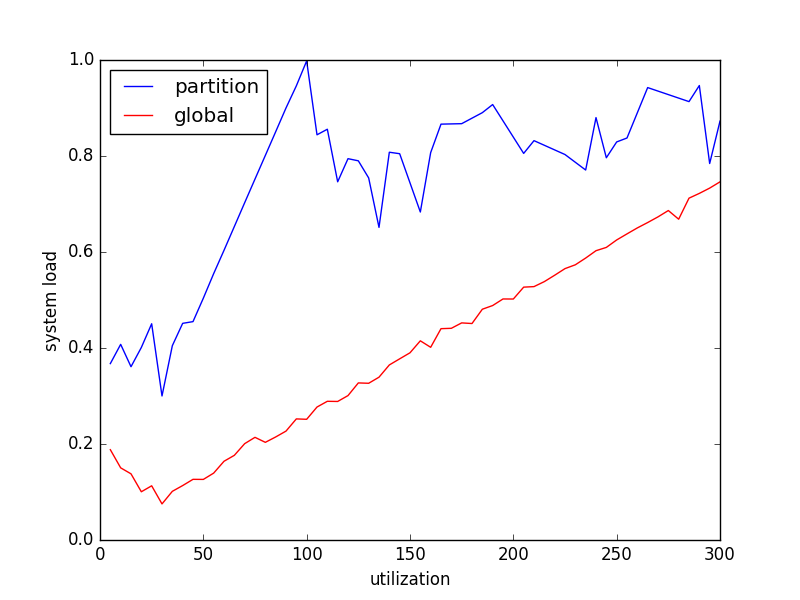
\includegraphics[width=0.4\textwidth]{plots/load_util_fixed.png}\label{fig:f1}}
  \hfill
  \subfloat[Minimum number of processors]{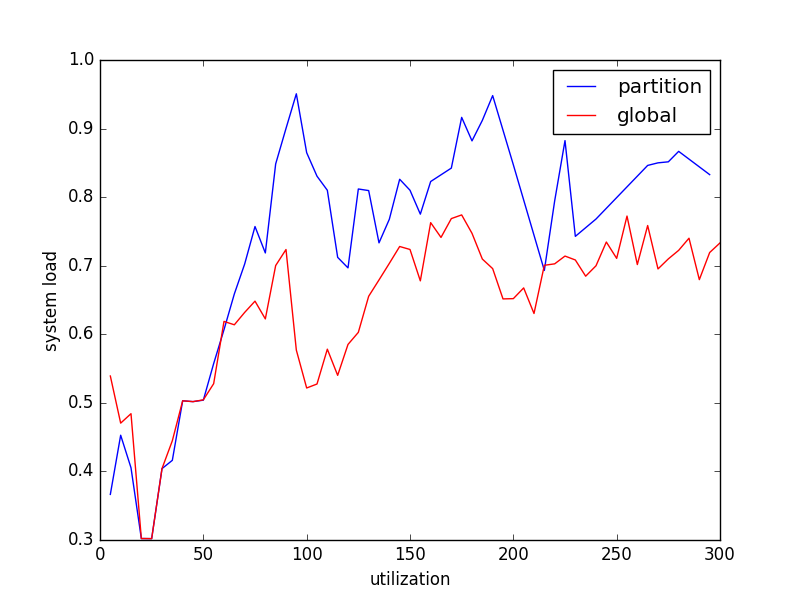
\includegraphics[width=0.4\textwidth]{plots/load_util_min.png}\label{fig:f2}}
  \caption{Load depending on utilization}
\end{figure}

\begin{figure}[H]
  \centering
  \subfloat[Fixed number of processors]{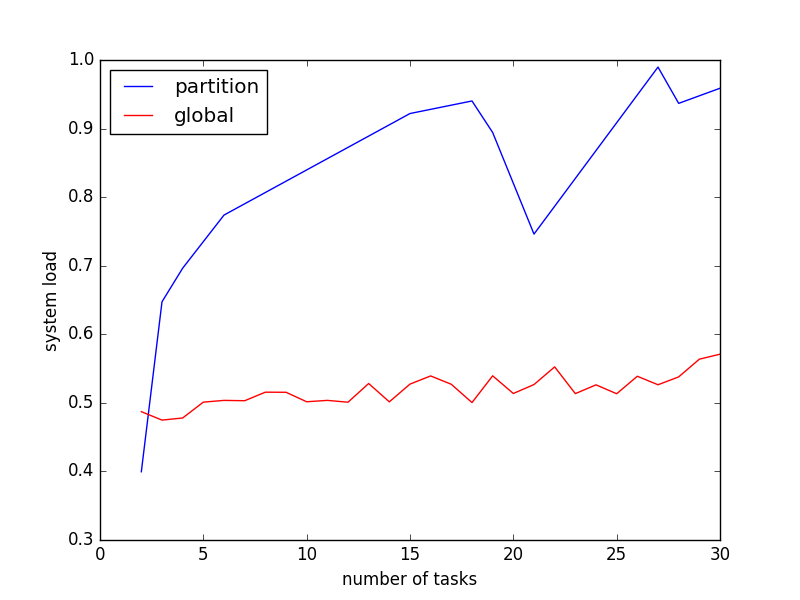
\includegraphics[width=0.4\textwidth]{plots/load_num_tasks_fixed.png}\label{fig:f3}}
  \hfill
  \subfloat[Minimum number of processors]{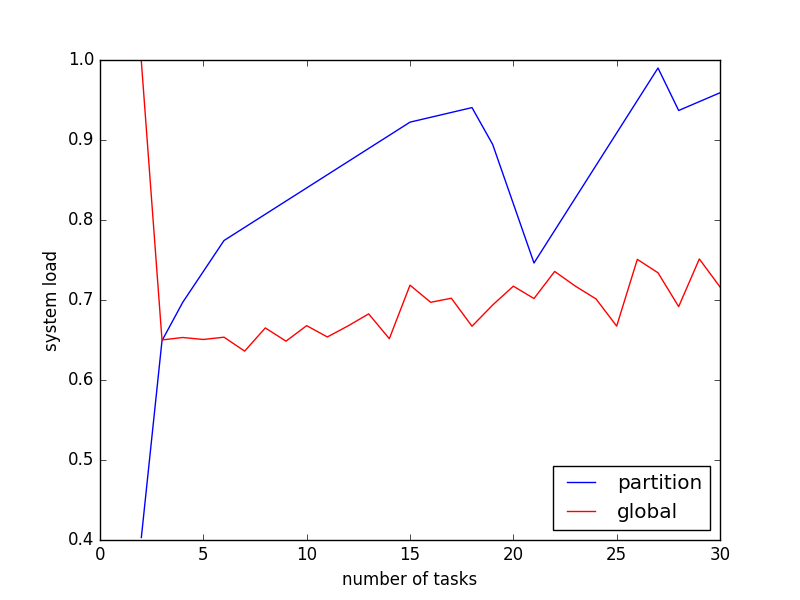
\includegraphics[width=0.4\textwidth]{plots/load_num_tasks_min.png}\label{fig:f4}}
  \caption{Load depending on number of tasks}
\end{figure}

\begin{figure}[H]
  \centering
  \subfloat[Depending on utilization]{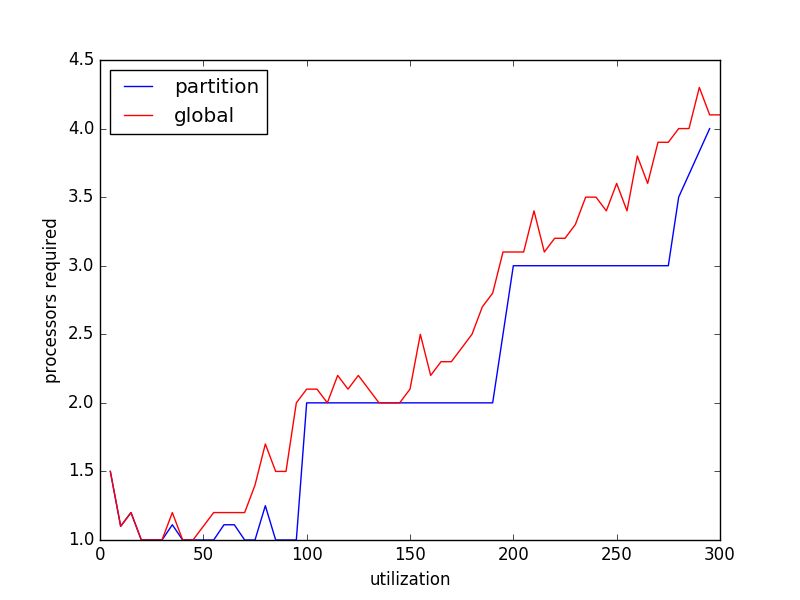
\includegraphics[width=0.4\textwidth]{plots/procs_util.png}\label{fig:f3}}
  \hfill
  \subfloat[Depending on number of tasks]{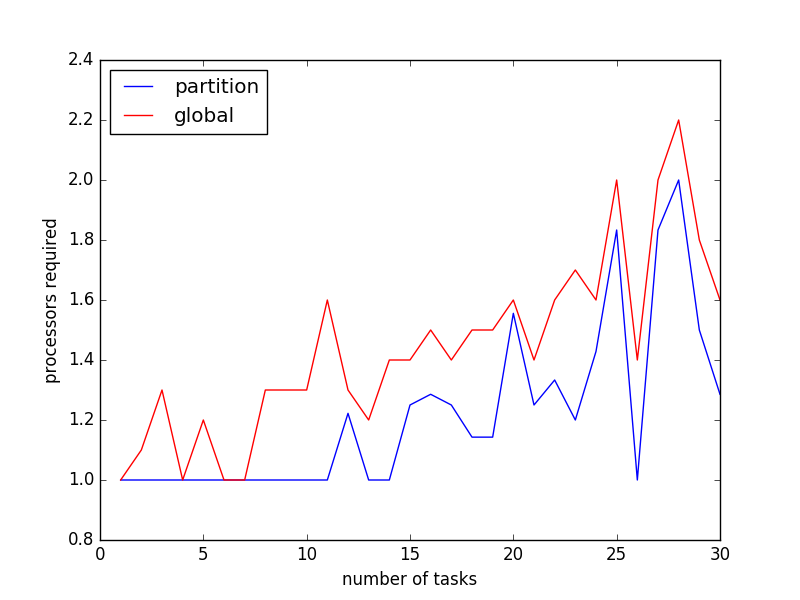
\includegraphics[width=0.4\textwidth]{plots/procs_num_tasks.png}\label{fig:f4}}
  \caption{Number of processors}
\end{figure}

\begin{figure}[H]
  \centering
  \subfloat[Depending on utilization]{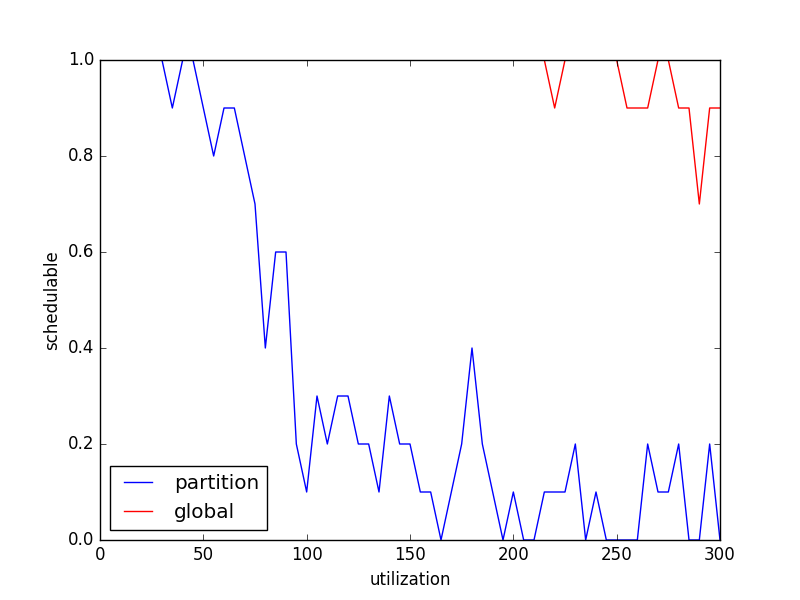
\includegraphics[width=0.4\textwidth]{plots/schedulable_util.png}\label{fig:f3}}
  \hfill
  \subfloat[Depending on number of tasks]{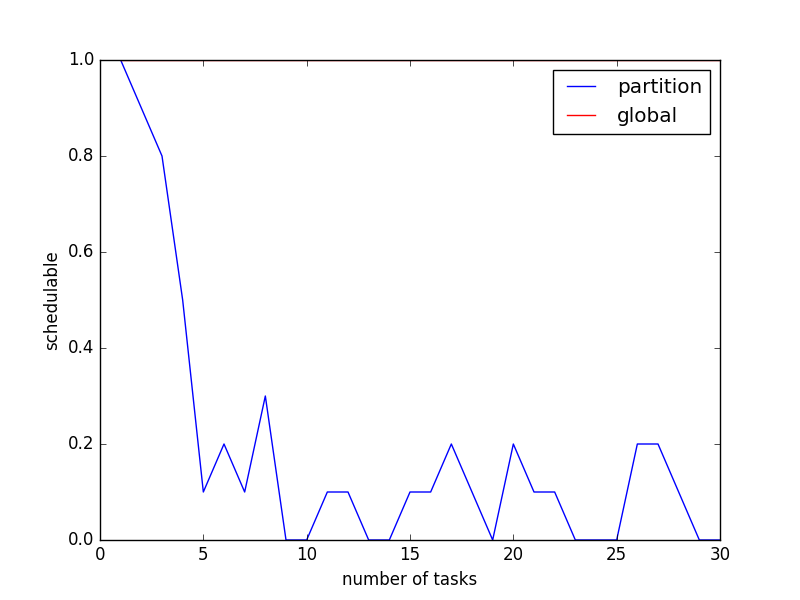
\includegraphics[width=0.4\textwidth]{plots/schedulable_num_tasks.png}\label{fig:f4}}
  \caption{Schedulability}
\end{figure}




\end{document}
